\documentclass[../thesis.tex]{subfiles}
\begin{document}

\chapter{Novel Blue Emitter Development}\label{sec:hoye}

Long lived deep blue emitters are important for developing displays.
This is still an active field of research.\supercite{Chan2018,Tang2018}
Despite extensive research and the transition of commercial red and green devices to phosphorescent materials, blue devices often utilize fluorescent emitters since phosphorescent emitters have a lower lifetime.\supercite{Scholz2015}
Because of the reduced efficiency, a larger blue fluorescent pixel is used than the corresponding red and green, in order to operate at a similar luminance point.
Though from an efficiency standpoint, a phosphorescent or TADF solution is the long term goal, there is still interest in developing high efficiency deep blue fluorescent emitters.\supercite{Lee2009b,Chi2010,Kim2008,Zhu2013,Lee2005}
This is especially true if novel chemistry can be used, producing entirely new classes of molecules.
Any new chemical understanding uncovered in fluorescent molecules may also be able to be transferred to phosphorescent molecules.

In this work, novel fluorescent emitter molecules were developed exhibiting deep blue emission.
Three distinct chemical families are investigated, all of which rely on synthesis through a hexadehydro-Diels-Alder (HDDA) cycloisomerization reaction.
The first set of these molecules focused around alkynyl substituted naphthalenes, work that was published in my work \textcite{Xu2016}.
The second set features  bis(arylethynyl) benzene derivatives..
The third presented set, though the first investigated, studies an arylethynyl fluorene.
All molecular synthesis in this chapter was conducted in the Prof. Thomas Hoye research group by Dr. Feng Xu.

\section{Hexadehydro-Diels-Alder Reactions}

The hexadehydro-Diels-Alder (HDDA) reaction is a method for producing aromatic compounds via cycloaddition.
Specifically, HDDA uses an alkyne (unsaturated hydrocarbon containing a carbon-carbon triple bond) and a diyne (system containing two alkyne groups) in order to form a reactive benzyne.
This benzene reacts with a trapping agent to form a substituted aromatic product.\supercite{Hoye2012,Yeoman2012}
Unlike conventional methods of preparation of benzenes, HDDA easily incorporates structural variations and substituents. \supercite{Bradley1997,Baire2013,Tadross2012} 
This makes HDDA a promising chemical method to produce conjugated, $\pi$-bond-rich molecules.
As discussed in Chapter \ref{sec:orgSemi}, conjugated molecules are of great interest as organic semiconductors.

\begin{wrapfigure}{r}{.5\textwidth}
\centering
\includegraphics[width=.48\textwidth]{hoye/hdda}
\caption{Preparation of benzenes through traditional Diels-Alder reaction (a) and an HDDA thermal cycloisomerization (b).  HDDA provides easy incorporation of substitutes at the A,B,C, Y and Z cites, along with the reactant (\textbf{7}).  Figure reproduced from \textcite{Xu2016}}
\label{fig:hoye_hdda}
\end{wrapfigure}


A schematic illustrating the advantages of HDDA reactions is shown in Figure \ref{fig:hoye_hdda}.
Figure \ref{fig:hoye_hdda}a shows a traditional method of production for naphthalene derivatives, starting from a benzenoid precursor (\textbf{1}).
Removing the X and Y substituents from (\textbf{1}), \textbf{2} can then be reacted with tetraphenylcyclopentadienone (TPCP) (\textbf{3}) via a Diels-Alder reaction.
After the thermal extrusion of carbon monoxide, naphthalene derivatives are formed (\textbf{4}).
In this process, it is difficult to incorporate substituents into the final product.
This is in contrast to the HDDA process shown in Figure \ref{fig:hoye_hdda}b.
Through HDDA thermal cycloisomerization of \textbf{5} into \textbf{6}, benzenes with complex substituents can be created.
Then through trapping with dienes like \textbf{7}, more complicated conjugated products can be realized.


Molecules were synthesized by Feng Xu in the Thomas Hoye research laboratory at the University of Minnesota.
Blue emission was seen under UV excitation, leading to characterization and collaboration with our group.


\section{Naphthalene Derivatives}\label{sec:hoye_nap}
\subsection{Synthesis}



The first molecular system studied used the reaction pathway shown in Figure \ref{fig:hoye_nap_reactions}.
Reactions between the tetraynes (\textbf{9}) and TPCP (\textbf{3}) via HDDA proceed through intermediates \textbf{11} and \textbf{12} before ejecting a carbon monoxide to form the fluorophores (\textbf{10}).\supercite{Giguere2015,Cacioppa2016,Pozo2016,Fieser1965,Wittig1958}
This HDDA cascade proceeded cleanly at 80 $\degree$C over the course of 12 hours and produced a yield of 82\% following three recrystallizations of the naphthalene adduct \textbf{10}. 
An added advantage of using a tetrayne substrate is that the intermediate benzene, here 11, and, consequently, the naphthalene formed following CO extrusion from 12, bears an arylethynyl substituent. 
The product \textbf{10a}, the first produced, showed strong emissive properties that were blue to the eye. 

\begin{wrapfigure}{r}{.5\textwidth}
\centering
\includegraphics[width=.48\textwidth]{hoye/nap_reactions}
\caption{HDDA reactions between \textbf{9} and \textbf{3} proceed through \textbf{11} and \textbf{12}, resulting in the products (\textbf{10}).  Figure reproduced from \textcite{Xu2016}}
\label{fig:hoye_nap_reactions}
\end{wrapfigure}

In light of these promising properties, the effect of the electronic character of the aryl substituents was probed. 
Two additional analogs in which the phenyl ring was modified by the presence of a pair of electron-donating (\textbf{10b}) as well as electron-withdrawing (\textbf{10c}) groups were prepared. 
These analogs were readily prepared by an entirely parallel and equally efficient sequence of reactions.



%\begin{wrapfigure}{r}{.5\textwidth}
%\centering
%\includegraphics[width=.48\textwidth]{hoye/nap_absorption_pl}
%\caption{Solution absorption (dashed lines) and emission (solid) at $10^{-5}$ M and $10^{-6}$ M, respectively, in THF.  Figure reproduced from \textcite{Xu2016}}
%\label{fig:hoye_nap_absorption}
%\end{wrapfigure}

Upon realization of fluorescence in the solid state, solutions were prepared in THF, to investigate their optical properties.
Absorption at $10^{-5}$M and photoluminescence at $10^{-6}$M are shown in Figure \ref{fig:hoye_nap_pl}.
A slight red shift in emission is seen for \textbf{10c} compared with \textbf{10a} and \textbf{10b}.
The PL quantum yield of each compound is summarized in Table \ref{tab:nap_pl}
\begin{wraptable}{r}{.35\textwidth}
\centering
    \begin{tabular}{|c|c|}
        \hline
        \textbf{Emitter} & \textbf{\pl (\%)} \\
        \hline
        \textbf{10a} & $11.0\pm2.6$ \\
        \textbf{10b} & $4.9 \pm 1.3$ \\
        \textbf{10b} & $56\pm8$\\
        \hline
    \end{tabular}
\caption{PL quantum yield (\pl)}
\label{tab:nap_pl}
\end{wraptable}
Given the promising solution PL efficiencies, the emissive properties of all three compounds were investigated in thin films to explore their possible utility as emissive species in blue organic light-emitting diodes (OLEDs). 

%\begin{wrapfigure}{r}{.5\textwidth}
%\centering
%\includegraphics[width=.48\textwidth]{hoye/nap_film_pl}
%\caption{ (a) Thin film PL from an 80/20 mixure of UGH2 and the emitter.  (b) Single crystal X-ray structure of \textbf{10b} showing the relative orientation in the solid state of all aryl substituents with respect to the core naphthalene ring.  Figure reproduced from \textcite{Xu2016}}
%\label{fig:hoye_nap_film_pl}
%\end{wrapfigure}
\begin{figure}[ht]
\centering
\includegraphics[width=.8\textwidth]{hoye/nap_pl_wide}
\caption{(a).Solution absorption (dashed lines) and emission (solid) at $10^{-5}$ M and $10^{-6}$ M, respectively, in THF. (b) Thin film PL from an 80/20 mixture of UGH2 and the emitter.  (c) Single crystal X-ray structure of \textbf{10b} showing the relative orientation in the solid state of all aryl substituents with respect to the core naphthalene ring.  Figure reproduced from \textcite{Xu2016} }
\label{fig:hoye_nap_pl}
\end{figure}

To probe thin film PL, each compound was examined both as a pure film (100\%) as well as in a host-guest arrangement with the wide energy gap material 1,4-bis(triphenylsilyl)benzene (UGH2) serving as host. 
Thin films were deposited on cleaned quartz substrates by high vacuum thermal evaporation ($10^{-7}$ Torr). 
Films composed of host and guest (UGH2 and \textbf{10}) in the ratios of 96:4, 80:20, and 0:100 (i.e., 4\%, 20\%, and 100\% loading, respectively) were studied. 
The thin film PL spectra of the 20\% samples of each of \textbf{10a-c} are shown in Figure \ref{fig:hoye_nap_pl}a. 
The solution and film emission maxima (Figures \ref{fig:hoye_nap_pl} and \ref{fig:hoye_nap_pl}b) are similar, suggesting that the excitonic state is unimolecular, without significant charge transfer states.
The twisted nature of the five aryl substituents on the central naphthalene ring as well as the quasi-orthogonal orientation of the pair of malonate carbomethoxy groups may be responsible for preventing close association between molecules of \textbf{10} in films. 
These features can be seen in the single crystal X-ray crystallographic structure shown in Figure \ref{fig:hoye_nap_pl}b. 
The PL emission spectra of all three compounds showed a red shift of between \textbf{10} and 20 nm across the extreme concentrations of 4\% vs 100\% content of \textbf{10}. 
This could be a result of at least some degree of aggregation with increasing concentration in the film, a response to a change in bulk dielectric properties or to differing intermolecular restraints that change the geometry of the excited states. 
DFT calculations (M06-2X/6-31G(d)) of the optimized lowest energy conformer for each of \textbf{10a-c} showed both the twisted the ethynyl linker, quite similar to those features seen for the single crystal, shown in the SI of \textcite{Xu2016}. 

\subsection{Performance Optimization}

\begin{wrapfigure}{r}{.5\textwidth}
\centering
\includegraphics[width=.48\textwidth]{hoye/nap_oleds}
\caption{(a) OLED architecture. (b)  EL spectra for \textbf{10a}. (c) EL spectra for \textbf{10b}. (d) EL spectra for \textbf{10c}.  Figure reproduced from \textcite{Xu2016}}
\label{fig:hoye_oleds}
\end{wrapfigure}

OLEDs using each of \textbf{10a-c} as the emissive layer were constructed by high vacuum thermal evaporation. 
Devices (Figures \ref{fig:hoye_oleds}a-c) were fabricated in accordance with our standard protocol.
The device architecture consisted of a 30 nm-thick hole transport layer (HTL) of 4,4'- cyclohexylidenebis[N,N-bis(4-methylphenyl)benzenamine] (TAPC), a 20 nm-thick emissive layer of \textbf{10a}, \textbf{10b},or \textbf{10c} doped into the wide energy gap host UGH2 at a concentration of 4, 20, or 100\% of the emitter, and a 30 nm-thick electron transport layer of tris(2,4,6-trimethyl-3-(pyridin-3-yl)phenyl)- borane (3TPYMB). 
All devices were capped with an electron- injecting cathode comprising a 0.5 nm-thick layer of LiF and a 100 nm-thick layer of Al. 
Electroluminescence (EL) intensity spectra collected for devices containing 20\% loading are shown in Figure \ref{fig:hoye_oleds}d. 
Data for devices containing a neat emissive layer of \textbf{10c} (Figure \ref{fig:hoye_oleds}d) show a significant red shift compared to the PL spectrum. 
We speculate that this emission may originate from an interfacial exciplex in this particular device. 
Upon doping with the UGH2 host, this effect is eliminated for the devices containing the 20\% and 4\% films. 

\begin{wraptable}{r}{.5\textwidth}
\centering
\begin{tabular}{ccccccc}
&&&&&CIE&\\
Emitter & Conc. & \eqe & \pl & $V_{TO}$ & x & y \\
\hline 
\textbf{10a} & 4 & 1.4 & 93.3 & 3.6 & 0.18 & 0.10 \\
& 20 & 3.0 & 42.9 & 3.5 & 0.15 & 0.09 \\
& 100 & 1.6 & 34.8 & 3.3 & 0.15 & 0.13 \\
\textbf{10b} & 4 & 0.9 & 51.1 & 3.8 & 0.18 & 0.11 \\
& 20 & 1.9 & 46.2 & 3.5 & 0.15 & 0.08 \\
& 100 & 1.9 & 43.0 & 3.1 & 0.15 & 0.10 \\
\textbf{10c} & 4 & 0.7 & 73.9 & 4.6 & 0.18 & 0.14 \\
& 20 & 0.9 & 56.6 & 3.6 & 0.15 & 0.17 \\
& 100 & 0.4 & 30.2 & 3.1 & 0.23 & 0.43
\end{tabular}
\caption{Summary of OLED device performance.  }
\label{tab:hoye_nap_perf}
\end{wraptable}

To evaluate spectral compatibility with display applications, the coordinate system describing the color gamut developed by the International Commission on Illumination (CIE) is used. 
Deep blue emission is required to reproduce fully the visible color spectrum for displays as well as to achieve true white colors. 
For application in television displays, desirable deep blue emission has CIE coordinates of x = 0.131, y = 0.04614a or x = 0.14, y = 0.08.
The coordinates observed for the above devices based on \textbf{10a-c} are reported in Table 1 (and graphically in Figure \ref{fig:hoye_cie}). 
All but the last (100\% \textbf{10c}) emit in the deep blue.

\begin{wrapfigure}{r}{.5\textwidth}
\centering
\includegraphics[width=.48\textwidth]{hoye/nap_cie}
\caption{CIE coordinates of OLEDs.  Circles, squares, and triangles are 4, 20 and 100\%, respectively. Closed, open, and plus represent \textbf{10a}, \textbf{10b}, and \textbf{10c}, respectively.  Figure reproduced from \textcite{Xu2016}}
\label{fig:hoye_cie}
\end{wrapfigure}

Current density-voltage and brightness-voltage characteristics were also measured for devices based on each emitter. 
From these measurements, the external quantum efficiency (\eqe) was calculated. 
The \eqe is a direct measure of photons emitted from the device in the forward viewing direction per electron injected.
Device performance for all emitter species and concentrations are shown in Table \ref{tab:hoye_nap_perf}. 
The highest performance device overall was found to be \textbf{10a} doped into UGH2 at 20\% with an \eqe of 3\%. 
It is worth noting that for simple fluorescent emitters, a maximum theoretical efficiency of 5\% is expected.\supercite{Yang2004,Kim2015}
Peak \eqe values for all three compounds are realized for devices having an emissive layer composition of 20\% of \textbf{10}. 
This does not correlate directly with the PL efficiency \pl, which increases monotonically with dilution, likely reflecting a role played by the emitter in charge transport. 
The wide energy gap of UGH2 (HOMO = 7.2 eV; LUMO = 2.8 eV)\supercite{Ren2004} forces charge transport to occur in part via the emissive guest molecule, especially for holes. 
This is supported by the observed increase in turn-on voltage ($V_{TO}$) with decreasing concentration. 
These devices could likely be further optimized by using a charge transporting host and a lower guest concentration, capitalizing on the improved PL efficiency observed for more dilute films.

\subsection{Electrical Lifetime}

\begin{wrapfigure}{r}{.5\textwidth}
\centering
\includegraphics[width=.48\textwidth]{hoye/nap_degraded_spectra}
\caption{Spectral degradation of \textbf{10b} under applied current. Spectra were taken in the order of the legend.}
\label{fig:hoye_nap_degraded_spectra}
\end{wrapfigure}

With reasonable device efficiencies, the primary motivation for fluorescent emitter development is to enhance lifetime.
It is notable that following deposition of each of the naphthalenes \textbf{10a-c}, there was virtually no residue remaining in the heating crucible, suggesting little if any thermal degradation of these compounds. 
In fact, this point could be preliminarily established for samples of \textbf{10a-c} by observing (i) their sublimation in common laboratory apparatus with essentially no decomposition and (ii) their robust nature when held open in the air at a temperature of $\le$300 $\degree$C, where they showed slight colorization but no sign of any significant decomposition. 
Finally, examination by differential scanning calorimetry again gave no indication of decomposition (exotherm) below 300 $\degree$C (for \textbf{10a} and \textbf{10b}) or 310 $\degree$C (for \textbf{10c}), and thermogravimetric analysis showed mass loss of greater than 5\% only at temperatures $>$336-357 $\degree$C (see SI of \textcite{Xu2016}). 

Despite these positive signs of thermal stability, devices showed a significant spectral shift under applied current.
Figure \ref{fig:hoye_nap_degraded_spectra} shows the degradation of \textbf{10b} as a function of increasing current.
As the current increases above 1 mA/cm$^2$, an additional spectral feature at 575 nm is seen developing.  
The intensity of the feature increases with current density.
This behavior is not reversible, and the intensity remains high even when returning to low current.  
Given the wide energy band of the host, it is unlikely that this is an exciplex with the host.
Additionally, since this is non-reversible, this is most likely a degradation state of the emitter.

\begin{wrapfigure}{r}{.4\textwidth}
\centering
\includegraphics[width=.38\textwidth]{hoye/nap_10c_lifetime}
\caption{Lifetime of molecule \textbf{10c}.}
\label{fig:hoye_10c_lifetime}
\end{wrapfigure}

With these positive indications from a molecular standpoint, lifetimes were investigated using NPD as an HTL and AlQ$_3$ as an ETL.
These materials were used to show higher stability, along with a neat EML of \textbf{10c} to avoid the instability of UGH2.
Unfortunately, the lifetimes shown in Figure \ref{fig:hoye_10c_lifetime} is very short at 4.7 hours, only operating at 7 cd/m$^2$.
This is an unusable lifetime for device applications.
Further optimization was not performed to improve lifetime.

\subsection{Solution Molecular Aggregation}

\begin{wrapfigure}{r}{.5\textwidth}
\centering
\includegraphics[width=.48\textwidth]{hoye/nap_pl_concentration}
\caption{\pl as a function of concentration THF in water.  Figure reproduced from \textcite{Xu2016}}
\label{fig:hoye_pl_concentration}
\end{wrapfigure}

Surprisingly, these compounds also showed a behavior typical of aggregation-induced emission (AIE). 
Namely, as the strong solvent THF was exchanged for increasing amounts of the non-solvent water, the efficiency of blue emission grew (see SI). 
However, given the array of five orthogonal aryl substituents, one would not expect that two (or more) molecules of \textbf{10} would be able to reside close enough to show substantial excimeric behavior. 
Perhaps the planar (arylethynyl)- naphthalene portion of the molecule provides enough of a footprint for close association of molecular orbitals from two molecules. 
We do note that a topologically related compound, 1- methyl-1,2,3,4,5-pentaphenylsilole, also shows significantly enhanced emission when placed under aggregate-inducing conditions.1

\section{Bis(arylethynyl) benzene Derivatives}\label{sec:hoye_triben}

\begin{wrapfigure}{r}{.5\textwidth}
\centering
\includegraphics[width=.35\textwidth]{hoye/triben_reactions}
\caption{Synthesis pathway. Precursors \textbf{b1} and \textbf{b2} undergo a HDDA reaction to form \textbf{b3}, and with the addition of the additional alkynyl, forms the product \textbf{b4}. Substituent variants R are shown.}
\label{fig:hoye_triben_reactions}
\end{wrapfigure}

A second molecular series was investigated, consisting of 1,4-bis(arylethynyl) benzene derivatives.
The synthesis for this series is depicted in Figure \ref{fig:hoye_triben_reactions}.
An HDDA reaction occurs between \textbf{b1} and a concentration of \textbf{b2} in excess of 3:1, resulting in \textbf{b3}.
With the further addition of another alkynyl group, the final products, \textbf{b4a} and \textbf{b4b} are formed.


The solution absorption and photoluminescence spectra of these compounds is shown in Figure \ref{fig:hoye_triben_pl}.  
The quantum yields of  \textbf{b4a} and \textbf{b4b}  were found to be $\pl=75.7\%$ and $\pl=81.2\%$, respectively.
Despite the high quantum yield in comparison to the molecules discussed in Section \ref{sec:hoye_nap}, the emission spectra is found to be limiting to applications.
Since the emission peak is below 400 nm for both materials, most emission is in the UV and would provide minimal visible output.
This would result in an extremely low luminance efficiency.
Therefore, devices using this molecular series were not further investigated.

\begin{figure}[ht]
\centering
\includegraphics[width=.48\textwidth]{hoye/triben_pl}
\caption{Photoluminescence spectra of compounds \textbf{b4a} and \textbf{b4b} shown in solid lines. Dashed lines show corresponding absorption spectra.}
\label{fig:hoye_triben_pl}
\end{figure}


\section{Arylethynylfluorene }\label{sec:hoye_bla}

\begin{wrapfigure}{r}{.5\textwidth}
\centering
\includegraphics[width=.48\textwidth]{hoye/oh_reactions}
\caption{The thermal HDDA reaction of tetrayne (\textbf{1}) affords the arylethynyldibenzofuran (\textbf{5}). The reaction proceeds through three reactive intermediates: benzene (\textbf{2}), zwitterion (\textbf{3}), and oxonium ion (\textbf{4}). Credit to Xiao Xiao for reaction diagram.}
\label{fig:hoye_oh_reactions}
\end{wrapfigure}

Molecules for this study were formed using the reaction shown in Figure \ref{fig:hoye_oh_reactions}.
Three different $R$ species were used, being OH, OMe, and COOMe.
The photoluminescence peak wavelength and efficiency can be found in Table \ref{tab:hoye_oh}.
Interestingly, in films and solution, the OMe molecule showed significant spectral changes based on the environment.
This seems to indicate that there is a large interaction between molecules, most likely due to the large planar conjugated system.
The OH molecule was expected to show similar behavior.
The COOMe system showed greed emission, and was not further investigated.

\begin{table}
\centering
    \begin{tabular}{ccc}
Molecule & $\lambda_{peak}$ (nm) & \pl (\%)\\
\hline \\
OH (neat) & 415 & 37 \\
OMe (neat) & 430 & 17 \\
OMe (20\% in UGH2) & 400 & 30 \\
COOMe (neat) & 500 & 33
    \end{tabular}
\caption{Photoluminescence summary for the emitter molecules of Figure \ref{fig:hoye_oh_reactions}}
\label{tab:hoye_oh}
\end{table}

In order to be useful, control over the emission wavelength needs to be obtained.
Devices utilizing OMe were further investigated to try to optimize spectral purity and device efficiency.
Four architectures were investigated, shown in Figure \ref{fig:oh_el_combo}I with the corresponding spectra shown in Figure \ref{fig:oh_el_combo}II.
The spectral feature at 375 nm closely reflects the dilute solution spectra for this molecule.  
The feature at 675 nm is a degradation product that increases in intensity after testing at high current.
It is unclear if this is a radiative degradation product or an exciplex formed with a degraded and undegraded molecule.
For both A and C, a broad aggregate emission state is seen at 430 nm.
Due to the lack of understanding of this emission state and wide variability in behavior, this molecular system was not deemed of further interest. 
The large planar conjugated state is thought to be the cause of this aggregate state emission, something which is avoided in the molecules discussed in Sections \ref{sec:hoye_nap} and \ref{sec:hoye_triben}.

\begin{figure}[ht]
\centering
\includegraphics[width=.8\textwidth]{hoye/oh_el_combo}
\caption{I. Architectures used for EL spectra optimization. II. El spectra for all devices reported at 2 mA/cm$^2$.}
\label{fig:oh_el_combo}
\end{figure}


% ``G:\My Drive\Group Meeting Presentations\16_01_04 hoye lifetimes.pptx''
% G:\My Drive\Group Meeting Presentations\2015\15_11_04 - hoye meeting.pptx



\section{Molecular Lifetime Screening}\label{sec:hoye_solutionPL}
Design rules for stable emitters are not well developed, so it is possible that closely related molecules could have a significant change in stability.
A rapid screening technique is needed to brute force optimize emitter molecules for lifetime since the stability cannot be predicted a priori.
Ideally, this technique would probe the intrinsic stability of the emitter, rather than the stability of an OLED device, as device manufacturing requires optimization of its own.
The most isolated molecular properties can be probed in solution, where molecules are not in contact with each other.
Solution has the added advantage of easy processing, further enabling rapid screening.

\begin{figure}[ht]
\centering
\includegraphics[width=.28\textwidth]{hoye/solutionPL}
\caption{Solution degradation setup for molecular screening.}
\label{fig:hoye_solutionPL}
\end{figure}

To investigate molecular lifetime, the solution photoluminescence degradation apparatus shown in Figure \ref{fig:hoye_solutionPL} was developed.
This setup uses a 375 nm fiber coupled LED as a pump, powered by a Keithley 26XX source meter.
When operated at the high luminance needed for a pump, UV LEDs suffer from low stability (interestingly, a related problem to the one we are trying to solve).
In order to operate at a constant pump dose during the test and between samples, a feedback loop is implemented using a split fiber.  
This fiber (blue in Figure \ref{fig:hoye_solutionPL}) has two cores, a large 1 mm diameter, as well as a 50 $\mu$m diameter.
The small core is used for the feedback loop to the power supply, adjusting the optical power every 5 minutes during the lifetime.
The large fiber is used to support the high light intensity needed to degrade the sample.


\begin{wrapfigure}{r}{.5\textwidth}
\centering
\includegraphics[width=.48\textwidth]{hoye/solutionPL_schem}
\caption{Schematic of the sample chamber for solution degradation.  1. Fiber coupled incoming light. 2. Beam Collimator. 3. Dark enclosure with nitrogen purge. 4. Expanded beam covering sample. 5. Cuvette. 6. 3x10 mm solution well. 7. Long pass filter to remove scattered laser light. 8. Photodiode. 9. Light from sample.}
\label{fig:hoye_solutionPL_sample}
\end{wrapfigure}
The sample is contained in the black box of Figure \ref{fig:hoye_solutionPL}, which supports a 1 cm by 1cm base dimensioned cuvette.
During this measurement, it is important to evenly degrade the molecules in the solution.
In an unstirred cuvette, it is likely that diffusion of molecules is slower than degradation, so it is important that the excitation condition is evenly applied.
Several steps were implemented to ensure this was true in the testing configuration.
Firstly, as the light passes through the sample, a Beer's law absorption profile creates a difference in the absorbed does between the incident and exiting plane.
Dilute solutions used for this study typically have low absorption, but to minimize this effect, a short light path length is preferred.
This is implemented by using a cuvette with inner dimensions of 10 mm by 3 mm, with the 3 mm to minimize the path length, as shown in Figure \ref{fig:hoye_solutionPL_sample}.
To minimize intensity differences across the face of the cuvette, an expanding beam collimator is used on fiber input.  
This takes the small area fiber input and collimates the beam over a diameter of $\approx$ 1 cm, spreading the beam across the full width of the cuvette.
The beam likely has spatial non-uniformity, but exciting the full width of the cuvette was deemed adequate.
Additionally, the cuvette is only filled partially, to ensure that all of the solution is in the beam.


The tested molecules require highly volatile solvents, so a screw top cuvette is used to minimize evaporation of the solvent.
Emitters are frequently sensitive to oxygen quenching, increasing non-radiative relaxation processes.\supercite{Endo2008,Schueppel2007,Baldo2000}
To avoid this, in addition to the sealed cap with sample preparation in a nitrogen glovebox, the sample chamber is kept under a positive nitrogen pressure using a constant purge, shown as the white plastic line coming into the sample chamber in Figure \ref{fig:hoye_solutionPL}.

\begin{wrapfigure}{r}{.5\textwidth}
\centering
\includegraphics[width=.48\textwidth]{hoye/stir}
\caption{Scatter in signal when stirring.  Despite the noise, notice the constant baseline.}
\label{fig:hoye_stir}
\end{wrapfigure}

Initial tests using this setup showed loss in the photoluminescence that was reversible by physical agitation of the sample.  
This suggested that the molecule is precipitating out of the solution, though no precipitate was visible due to the dilute loading ($10^{-6}$ M).
Because of this, stirring needed to be added to the solution, and was done by adding a spherical stir ball and placing the apparatus on a stir plate.
However, the addition of the stir bar added significant noise to the measured PL signal, shown in Figure \ref{fig:hoye_stir}.
It was found that the movement of the stir bar caused significant scattering of the light and was impacting the measurement.
In addressing this problem, points were taken every 5 ms to observe the scatter.
It was found that a minimum signal was reliably achieved every 300 measurements.
This is believed to be a period where the stir bar is out of the light path and not scattering light.  
To eliminate the noise, 300 points are taken at 5 ms intervals, and the minimum is taken as the solution signal.

This method has been developed and is able to produce reliable results on the same solution.
Test results have started using FIr(pic) as an emitter.
Molecular screening has yet to be done using this technique.


\section{Conclusion}
This chapter outlined progress on three families of emitter molecules for blue fluorescent OLEDs.
Promising efficiency results were seen for the naphthalene derivatives, though the lifetime was found to be extremely short.
Without a promising lifetime, further development was not pursued.
A solution based molecular stability test was pursued in Section \ref{sec:hoye_solutionPL}.

The remaining two molecular families were eliminated from further investigation in the initial screening of photoluminescence.
It is very important for OLED device design to have a reliable emission state that can be confined.  
This was found to be challenging due to molecular aggregation and charge-transfer states in Section \ref{sec:hoye_bla}.
The molecules in Section \ref{sec:hoye_triben} emitted in the UV and were of minimal interest for OLED devices.


\ifcsdef{mainfile}{}{\printbibliography}
\end{document}
